\documentclass{beamer}

\usepackage{paratype}
\setbeamerfont{frametitle}{family=\bf}

% Beamer theme settings
\usecolortheme{seagull}
\usenavigationsymbolstemplate{} % no navigation buttons

\usepackage[utf8]{inputenc}

\title{OpenCL day 1: GPU hardware and the programming model}

\author{Cosmin Oancea and Troels Henriksen}

\date{January 28, 2019}

\begin{document}

\frame{\titlepage}

\section{Introduction and Course Contents}

\begin{frame}
  \tableofcontents[currentsection]
\end{frame}

\section{Hardware Trends}

\begin{frame}
	\tableofcontents[currentsection]
\end{frame}

\begin{frame}
  \frametitle{A graph of CPU progress}

  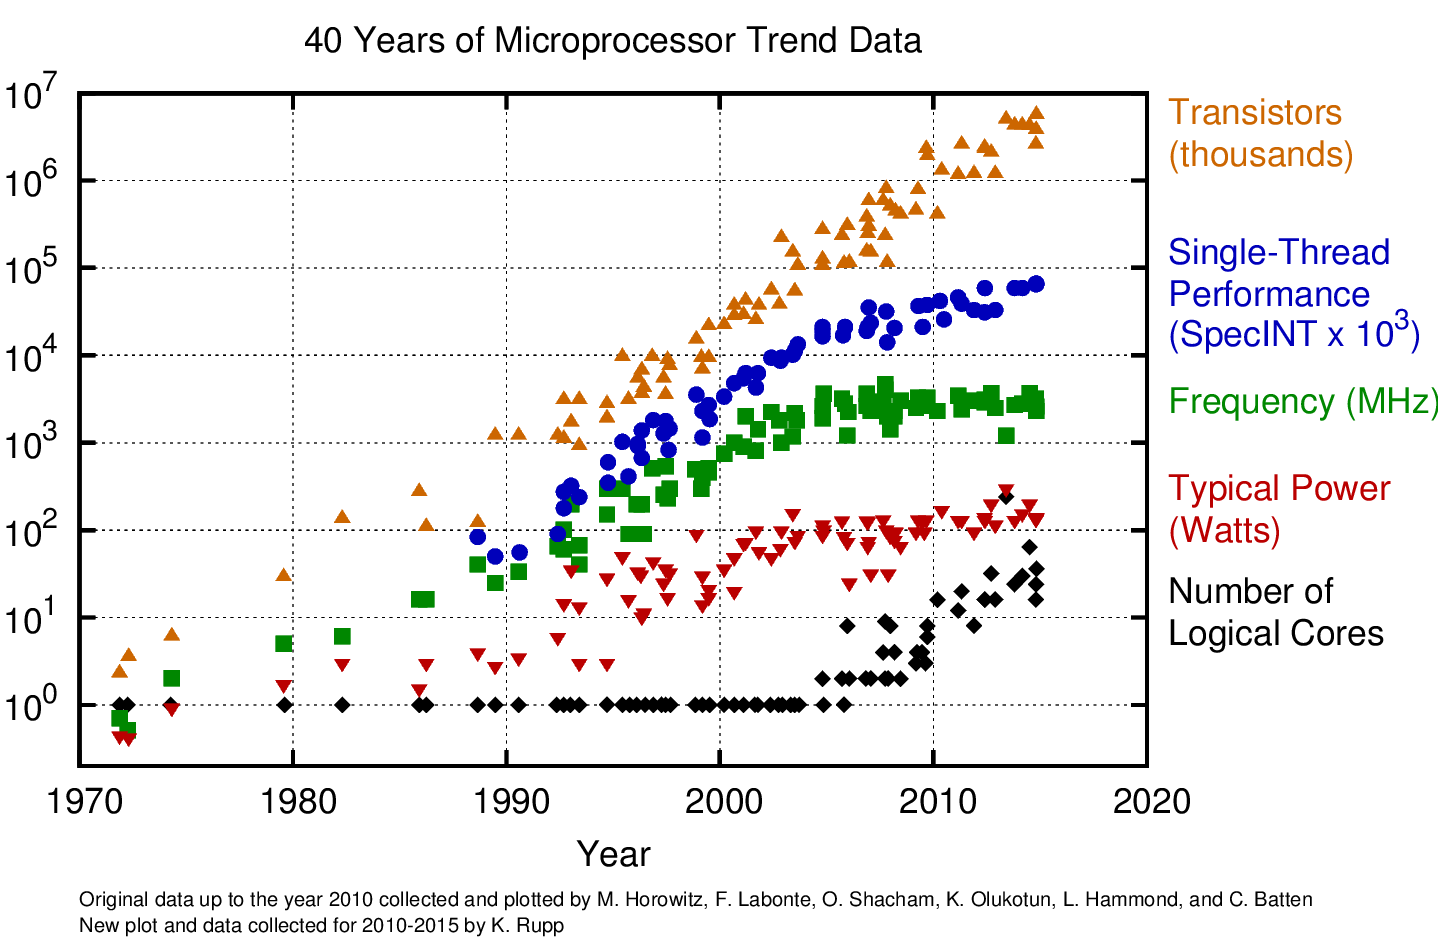
\includegraphics[width=\textwidth]{img/40-years-processor-trend.png}

\end{frame}

\section{CPU vs GPU architectures}

\begin{frame}
	\tableofcontents[currentsection]
\end{frame}

\begin{frame}
  \frametitle{GPUs vs CPUs}

  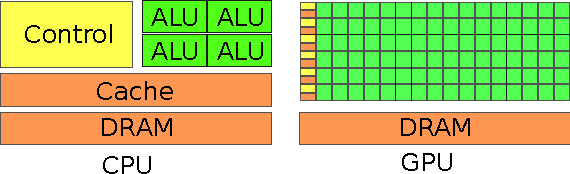
\includegraphics[width=\textwidth]{img/cpu-gpu-architecture.pdf}

  \begin{itemize}
  \item GPUs have \textit{thousands} of simple cores and taking full
    advantage of their compute power requires \textit{tens of
      thousands} of threads.
  \item GPU threads are very \textit{restricted} in what they can do:
    no stack, no allocation, limited control flow, etc.
  \item Potential \textit{very high performance} and \textit{lower
      power usage} compared to CPUs, but programming them is
    \textit{hard}.
  \end{itemize}

  \textbf{Massively parallel processing is currently a special case,
    but will be the common case in the future.}
\end{frame}

\section{The OpenCL programming model}

\begin{frame}
	\tableofcontents[currentsection]
\end{frame}

\section{Debugging and Profiling OpenCL}

\begin{frame}
	\tableofcontents[currentsection]
\end{frame}

\section{Programming Exercises}

\begin{frame}
	\tableofcontents[currentsection]
\end{frame}


\end{document}

%%% Local Variables:
%%% mode: latex
%%% TeX-master: t
%%% End:
